\section{Actividad 8}

\subsection*{En un determinado circuito se tienen tres amplificadores conectados en cascada, tal
como se puede observar en la Fig. }

    \begin{figure}[H]
        \centering
        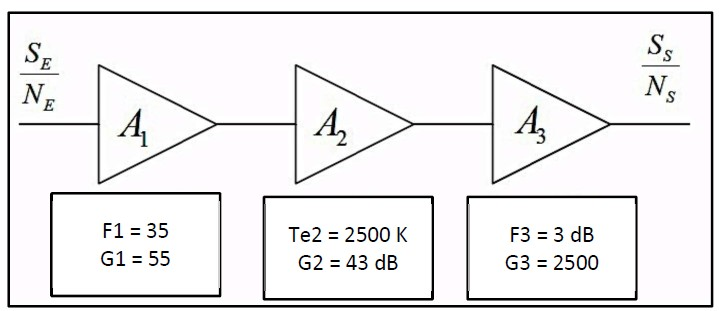
\includegraphics[width=0.8\linewidth]{imagenes/Actividad_8/actividad_8.jpg}
        \caption{Circuito en cascada.}
        \label{fig:diagrama_8}
    \end{figure}

\subsection*{Calcular:}

\subsection*{a) La figura de ruido total, suponiendo la temperatura ambiente T = 290 K.}


	Se procede a convertir los datos a la escala lineal ya que estos deberán de estar en una misma escala. Por lo tanto, se obtiene que:
	
	\begin{itemize}
		\item $ F_2 = \frac{290 [K] + 2500 [K]}{290 [K]} = 9,62$
		\item $ G_2 = 10^\frac{43}{10} = 19952,62315$
		\item $ F_3 = 10^\frac{3}{10} = 1,99526$
	\end{itemize}
	
	La figura de ruido total se calcula como:
	
	\[
		F = F_1 + \frac{F_2 - 1}{G_1} + \frac{F_3 - 1}{G_1 G_2}
	\]

	Reemplazando los valores correspodientes se obtiene que la figura de ruido total es: 
	
	\[
		F = 35 + \frac{9,62 -1}{55} + \frac{1,99526 - 1}{55 * 19952,62315} = 35,1567
	\]






\subsection*{b) La temperatura equivalente de ruido total.}

	Para realizar el cálculo de la temperatura equivalente de ruido total, la temperatura de cada amplificador deberá de estar en grados kelvin. Por lo tanto, al realizar dicha conversion se obtiene que:
	
	\begin{itemize}
		\item $ T_1 = T*(F_1 - 1) = 290 [K]*(35 -1) = 9860 [K]$
		\item $ T_3 = T*(F_3 - 1) = 290[K]*(10^\frac{3}{10} -1) = 288,6261 [K] $
	\end{itemize}

	La temperatura equivalente de ruido total se calcula como:
	
	\[
		T_e = T_1 + \frac{T_2}{G_1} + \frac{T_3}{G_1 * G_2}
	\]
	
	Al reemplazar los valores correspondientes se obtiene que la temperatura de ruido total es:
	
	\[
		T_e = 9860 [K] + \frac{2500 [K]}{55} + \frac{288,6162 [K]}{55 * 19952,62315} = 9905,455 [K]
	\]


\subsection*{c) Intercambiar los amplificadores A1 y A3. Calcular nuevamente la figura de ruido total, y explicar que sucede.}

	Al intercambiar los amplificadores $A_1$ y $A_3$ la ecuación de la figura de ruido total es:
	
	\[
		F = F_3 + \frac{F_2}{G_3} + \frac{F_1}{G_3 * G_2}
	\]
	
	Reemplazando los datos de los incisos anteoriores se obtiene que la nueva figura de ruido total es:
	
	\[
		F = 1,99526 + \frac{9,62}{2500} + \frac{35}{2500 * 19952,63215} = 1,999
	\]
	
	Al comparar éste nuevo resultado con el obtenido en el inciso a) se observa que el valor de la nueva figura de ruido total disminuye con respecto a la del inciso a). Por lo tanto, se concluye que para obtener una figura de ruido pequeña, la primer etapa de la conexión en cascada deberá tener una alta ganancia, además también se concluye que la figura de ruido total $F$ es dominada por la figura de ruido de la primer etapa.\par 
	
	
	
	

\subsection*{d) Suponer que ingresa a la cascada de amplificadores una señal con una potencia de 20x10-9 W. Calcular la relación señal ruido 
	tanto en la entrada, como en la salida de dicha cascada, considerando $\Delta f = 150 kHz$.}
	
	
	La potencia de ruido disponible a la entrada del circuito se calcula como:
	
	\[
		N_1 = k*T*\Delta f
	\]
	
	donde:
	
	\begin{itemize}
		\item $K = 1,380649x10^{-23} [\frac{J}{K}]$.
		\item $\Delta f$ es el ancho de banda estrecho centrado en $f$.
		\item $T$ es la temperatura ambiente en grados kelvin [K] 
	\end{itemize}
	
	Al reemplazar dichos valores se obtiene que la potencia de ruido disponible a la entrada es:
	
	\[
		N_1 =1,380649x10^{-23} [\frac{J}{K}]*290 [K]*150 [kHz] = 6,0058x10^{-16} [W]
	\]

	Realizando el cociente entre la señal de potencia $20x10^{-9} [W]$ a la entrada que ingresa al circuito con la potencia de ruido a la entrada $N_1$ se obtiene la relación 
	señal-ruido de la entrada de la fuente $SNR_s (f)$. Por lo tanto, se obtiene que:
	
	\[
		SNR_s (f) = \frac{20x10^{-9} [W]}{6,0058x10^{-16} [W]} = 33,3011x10^7.
	\]
	
	La figura de ruido total se puede expresar como:
	
	\[
		F = \frac{SNR_s (f)}{SNR_o (f)}
	\]
	
	Despejando $SNR_o (f)$ y reemplazando los datos se obtiene que la relación señal-ruido $SNR_o (f)$ en la salida es:
		
	\[
		SNR_o (f) = \frac{SNR_s (f)}{F} = \frac{33,3011x10^7}{35,156} = 9,4722
	\]
	
	
	